\section{Semaine 17 : 29/05/2023 - 02/06/2023}
\graphicspath{{semaines/semaine_17/images/}}

\begin{abstract}
	Cette semaine était assez courte. En effet, lundi était férié et le jeudi et le vendredi, il y a eut le déménagement.
	Globalement, cette semaine j'ai relancé mes résultats pour Legendre (avec les coefficients calculés sous formes matriciels). J'ai testé pour différents $P$ et ait considéré 3 types d'erreurs.
\end{abstract}

\subsection{Résultats FNO}

Cette semaine, on va essayer d'approcher par série de polynômes de Legendre directement la solution prédite (c'est-à-dire la sortie du FNO multipliée par la levelset $\phi$). On considérera
$$\widetilde{\alpha_{P,Q}}=\frac{4}{(N-1)(M-1)}\widetilde{D_P}^{-1}\widetilde{P_N}^T\widetilde{F_{N,M}}\widetilde{P_M}\widetilde{D_Q}^{-1}$$ 
En fait on ne multiplie pas réellement par $P_N^T$ à gauche mais par une matrice $P_N^{T,-}$ qui est égale à $P_N^T$ avec sa dernière colonne nulle. De la même manière, on ne multiplie pas réellement par $P_M$ à droite mais par une matrice $P_M^{-}$ qui est égale à $P_M$ avec sa dernière ligne nulle. 
On considérera les trois erreurs suivantes :
\begin{itemize}
	\item max(|Y\_pred-Y\_pred\_reconstruct|) -> errors\_reconstruct
	\item max(|(Y\_pred-Y\_pred\_reconstruct)*mask|) -> errors\_reconstruct\_mask
	\item $||Y\_test-Y\_pred\_reconstruct||_{L^2}$  -> errors\_legendre
\end{itemize}

\textit{Résultats :}

On considère $\Omega$ le cercle de rayon $\sqrt{2}/4$ et de centre $(0.5,0.5)$ avec $\Phi(x,y)=1/8-(x-1/2)^2-(y-1/2)^2$ et le domaine fictif $O=(0,1)^2$.
On prend
$$f(x,y) = \exp\left(-\frac{(x-\mu_0)^2 + (y-\mu_1)^2}{2\sigma^2}\right)\,, $$ 

On considère $N=M=599$ (=2*nb\_vert-1 avec nb\_vert=300).

Voici les 3 types d'erreurs obtenus pour $P=Q=4$ :

\begin{minipage}{\linewidth}
	\centering
	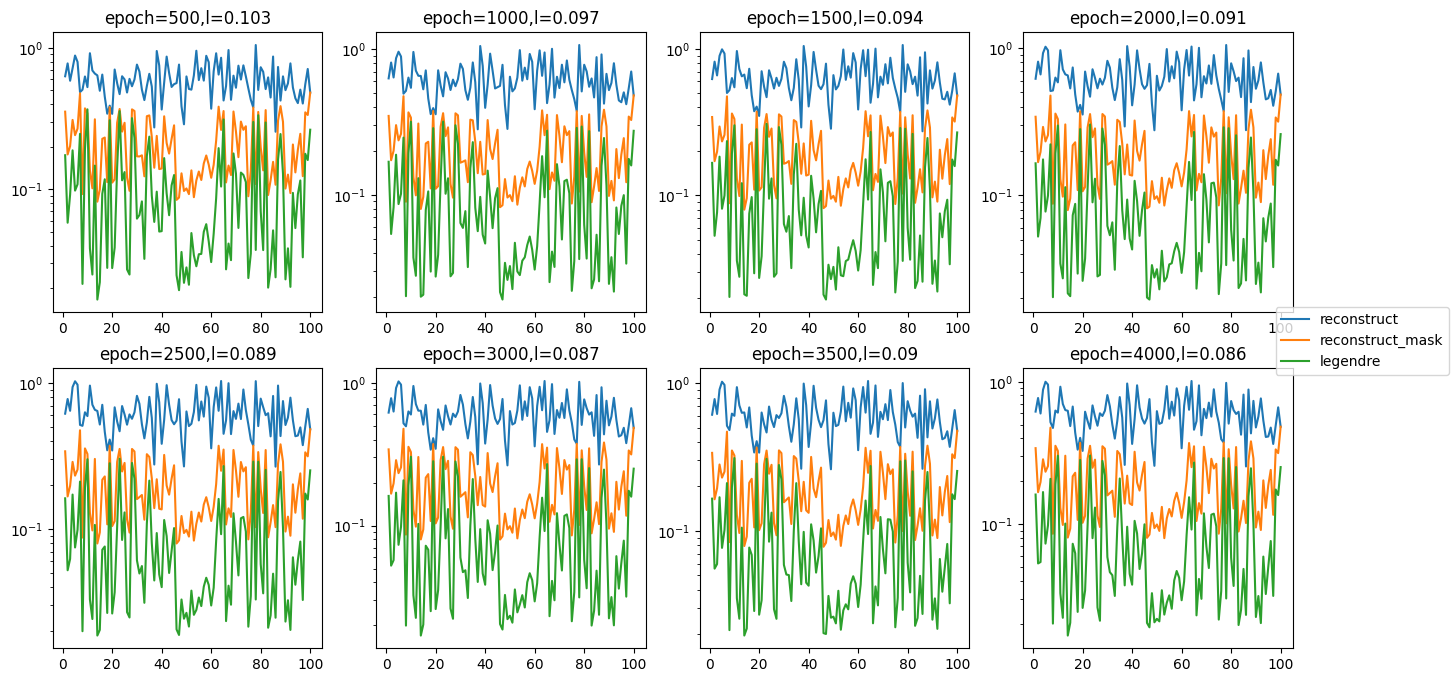
\includegraphics[width=0.7\linewidth]{errors_3_P4.png}
\end{minipage}

Voici également les résultats pour epoch=0 et data=0 :

\begin{minipage}{\linewidth}
	\centering
	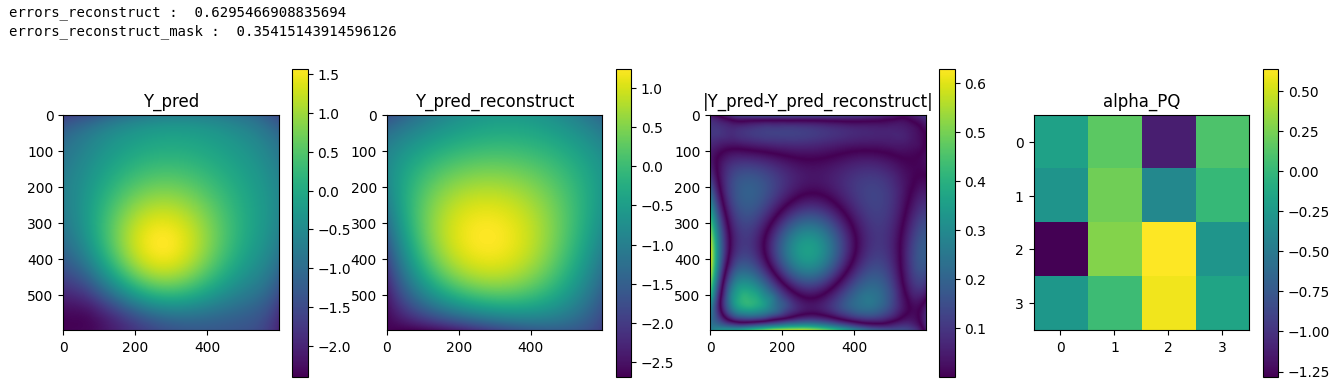
\includegraphics[width=0.8\linewidth]{example_P4.png}
\end{minipage}

\newpage

En testant pour différents P ($P\in\{4,6,8\}$), on obtient les résultats suivants :

\begin{minipage}{\linewidth}
	\centering
	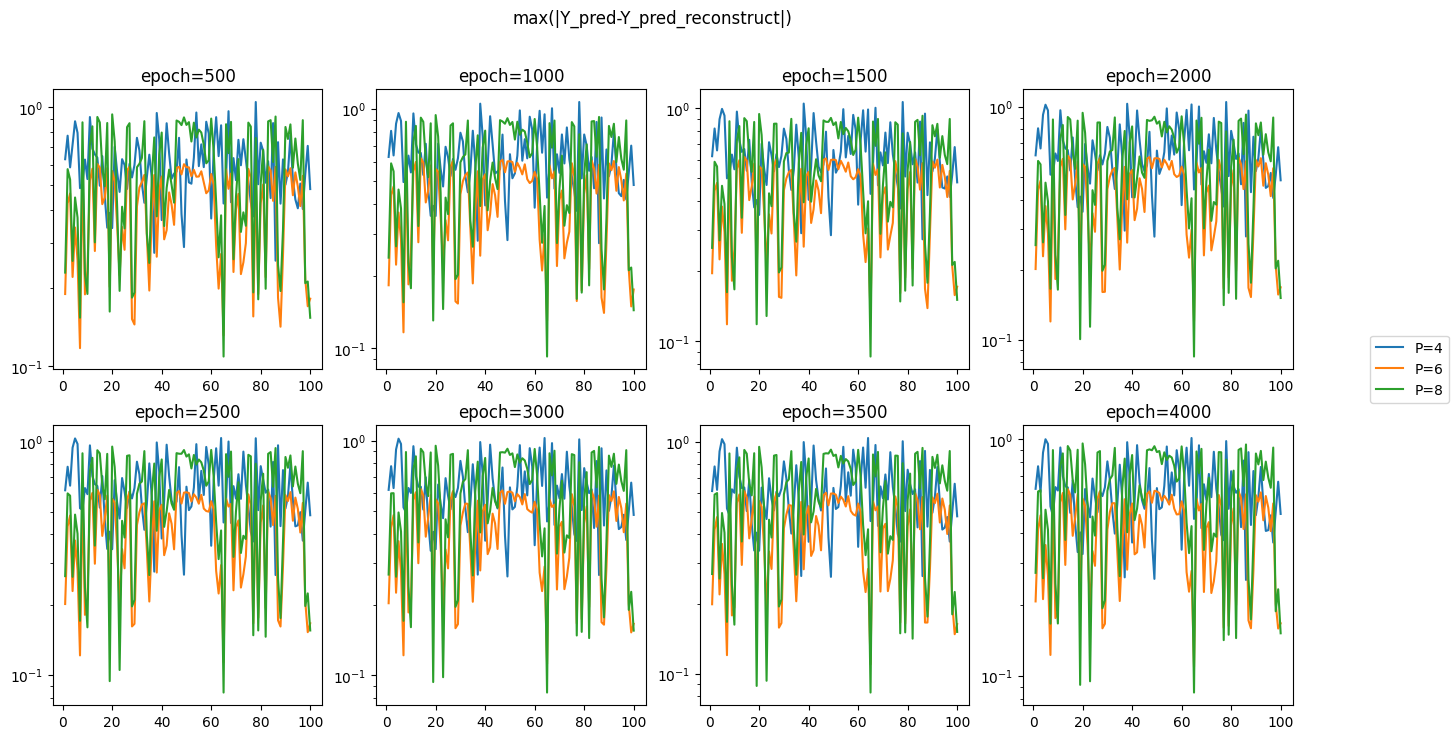
\includegraphics[width=0.7\linewidth]{errors_reconstruct.png}
\end{minipage}


\begin{minipage}{\linewidth}
	\centering
	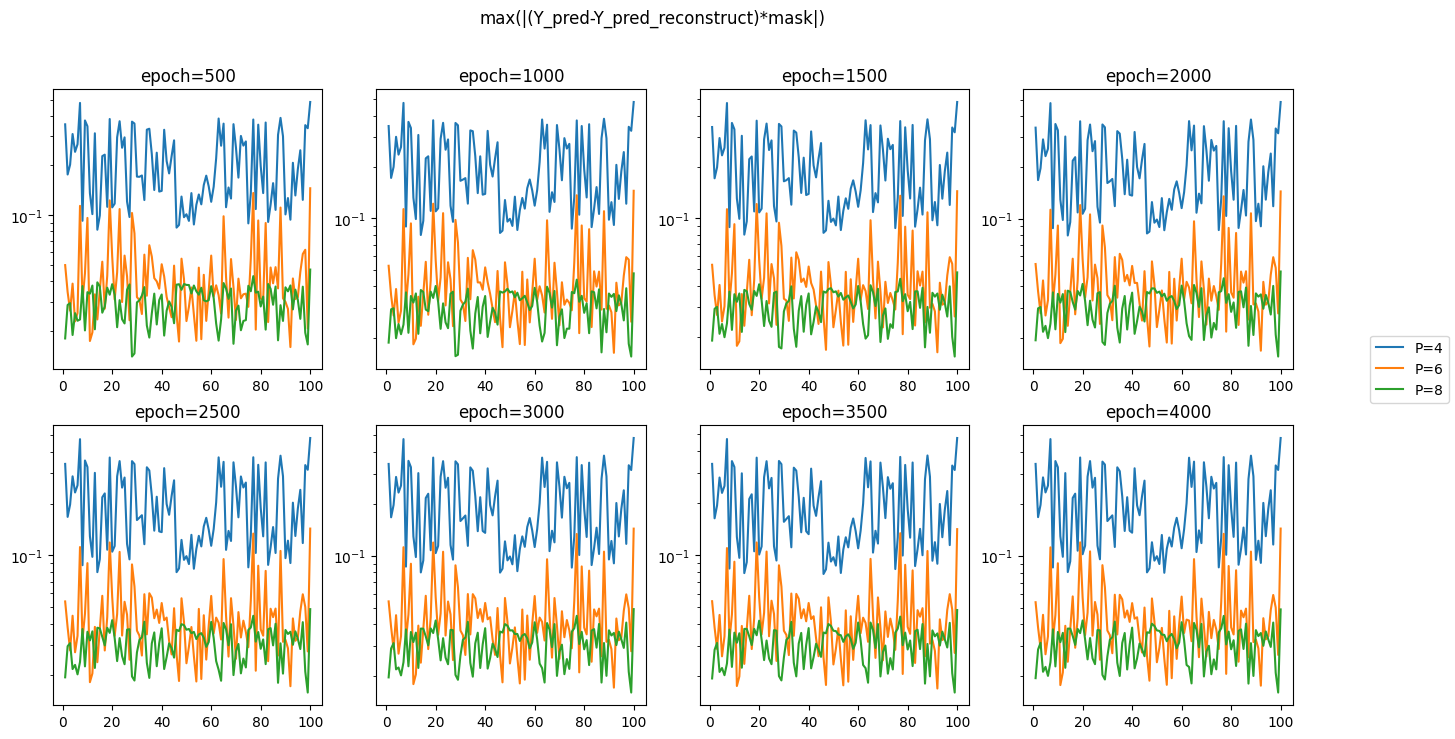
\includegraphics[width=0.7\linewidth]{errors_reconstruct_mask.png}
\end{minipage}


\begin{minipage}{\linewidth}
	\centering
	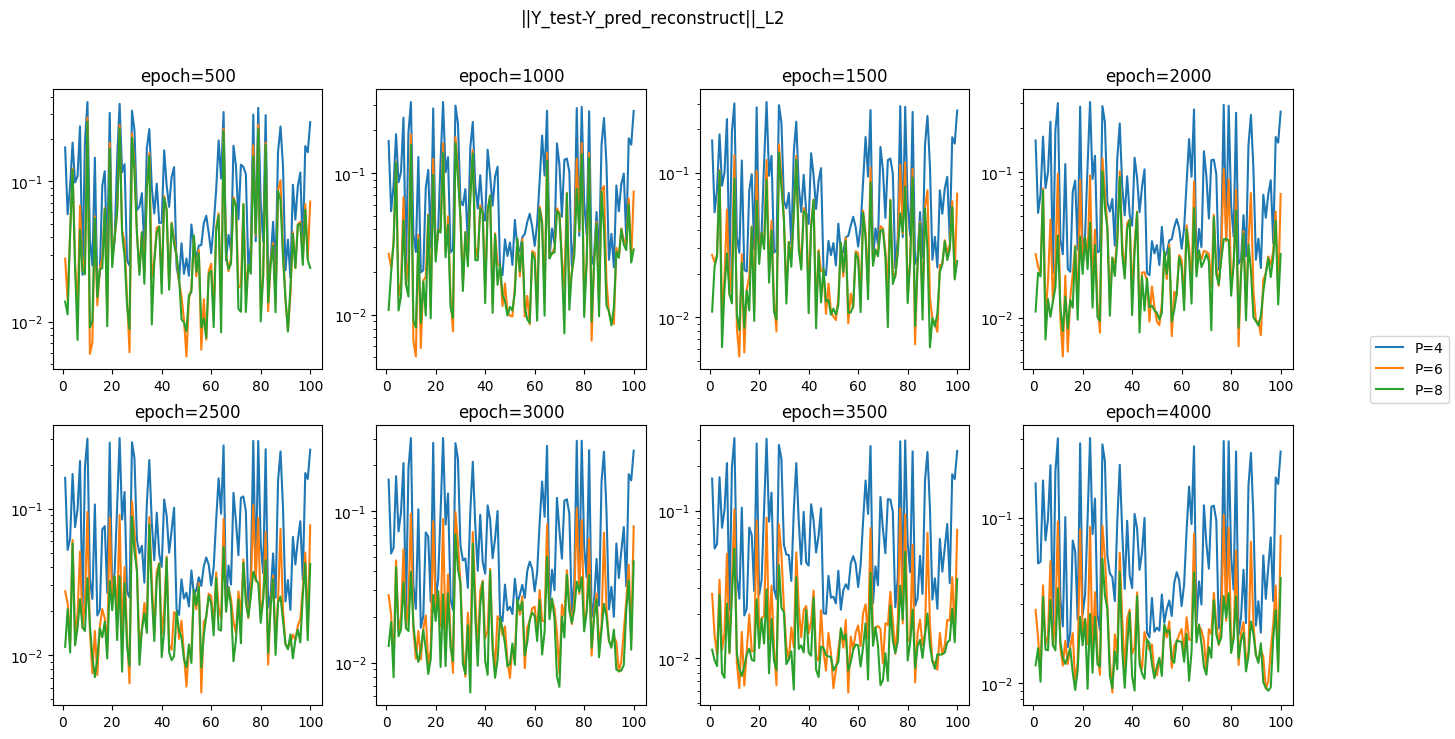
\includegraphics[width=0.7\linewidth]{errors_legendre.png}
\end{minipage}

\conclusion{Les résultats n'étant pas très bon, je pense qu'il serait mieux d'approcher $w$ par série de polynôme de Legendre plutôt que $u$ afin d'éviter les erreurs au bord du domaine. Je pense également qu'un problème est le changement de variable (sur la solution analytique ça ne fonctionne pas non plus en considérant les problèmes matriciels.)}